
\جزوحصہ{سطح حرکت پر ایک درجی مساوات میں تبادلہ}
سطح حرکت کی دوسری ترکیب خود مختار [جس میں \عددیء{t} صریحاً نہیں پایا جاتا] دو درجی سادہ تفرقی مساوات
\begin{align*}
F(y,y',y'')=0
\end{align*}
میں \عددی{y=y_1} کو آزاد متغیرہ اور \عددی{y'=y_2} لے کر \عددی{y''} کو زنجیری تفرق سے
\begin{align*}
y''=y_2'=\frac{\dif y_2}{\dif t}=\frac{\dif y_2}{\dif y_1}\frac{\dif y_1}{\dif t}=\frac{\dif y_2}{\dif y_1}y_2
\end{align*}
لکھ کر ایک درجی مساوات
\begin{align}
F\left(y_1,y_2,\frac{\dif y_2}{\dif y_1}y_2\right)=0
\end{align}
میں تبدیل کرنے پر مبنی ہے۔اس ایک درجی مساوات کو یا تو حل کرنا ممکن ہوتا ہے اور یا \اصطلاح{میدان ڈھال}\فرہنگ{میدان!ڈھال}\فرہنگ{ڈھال!میدان} کی مدد سے اس پر غور ممکن ہوتا ہے۔ آئیں مثال \حوالہ{مثال_نظام_دھاگے_سے_لٹکی_کمیت} پر اس ترکیب کی مدد سے غور کریں۔
%==========

\ابتدا{مثال}\شناخت{مثال_نظام_بلا_تقصیر_ارتعاش_یک_درجی_مساوات}\quad بلا تقصیر ارتعاشی نظام کی ایک درجی تفرقی مساوات۔\\
مساوات \حوالہ{مساوات_نظام_غیر_خطی_ترکیب_مرحلہ_ت} میں \عددی{\theta''+k\sin \theta=0} ہے جس میں \عددی{\theta=y_1} اور  \عددی{\theta'=y_2} (زاویائی رفتار) لیتے ہوئے
\begin{align*}
\theta''=\frac{\dif y_2}{\dif t}=\frac{\dif y_2}{\dif y_1}\frac{\dif y_1}{\dif t}=\frac{\dif y_2}{\dif y_1}y_2
\end{align*}
لکھ کر \عددی{\tfrac{\dif y_2}{\dif y_1}y_2=-k\sin y_1} ملتا ہے جس کو علیحدگی متغیرات سے \عددی{y_2\dif y_2=-k\sin y_1\dif y_1} لکھا جا سکتا ہے جس کا تکمل
\begin{align}\label{مساوات_نظام_کل_توانائی_الف}
\frac{1}{2}y_2^2=k\cos y_1+C 
\end{align}
دیتا ہے جہاں \عددی{C} تکمل کا مستقل ہے۔اس کو \عددی{mL^2} سے ضرب دینے سے
\begin{align*}
\frac{1}{2}m(Ly_2)^2-mL^2k\cos y_1=mL^2C
\end{align*}
حاصل ہوتا ہے جس کے تینوں اجزاء \اصطلاح{توانائی}\فرہنگ{توانائی}\حاشیہب{energy}\فرہنگ{energy} کو ظاہر کرتے ہیں۔چونکہ \عددی{y_2} زاویائی رفتار ہے لہٰذا \عددی{Ly_2} لمحاتی رفتار اور  \عددی{\tfrac{1}{2}m(Ly_2)^2} \اصطلاح{حرکی توانائی}\فرہنگ{حرکی توانائی}\فرہنگ{توانائی!حرکی}\حاشیہب{kinetic energy}\فرہنگ{energy!kinetic} ہے۔درج بالا مساوات کا دوسرا جزو (بمع منفی علامت) \اصطلاح{مخفی توانائی}\فرہنگ{توانائی!مخفی}\فرہنگ{مخفی توانائی}\حاشیہب{potential energy}\فرہنگ{energy!potential} ہے جبکہ مساوات کا دایاں ہاتھ \عددی{mL^2C} کل توانائی ہے۔بلا تقصیر نظام میں توانائی کا ضیاع نہیں پایا جاتا لہٰذا حزب توقع کل توانائی مستقل مقدار ہے۔آئیں دیکھیں کہ حرکت کی نوعیت کل توانائی پر کیسے منحصر ہے۔

شکل \حوالہ{شکل_مثال_نظام_دھاگے_سے_لٹکی_کمیت}-ب مختلف \عددی{C} کے لئے خط حرکت دیتی ہے۔ان خطوط کا دوری عرصہ \عددی{2\pi} ہے۔ان میں ترخیمی بند دائرے اور  لہر نما خطوط شامل ہیں جن کے مابین نقطہ زین [\عددی{(n\pi,0)} جہاں \عددی{n=\mp1,\mp3,\cdots} ہے] سے گزرتے ہوئے دو عدد خط حرکت  پائے جاتے ہیں۔مساوات \حوالہ{مساوات_نظام_کل_توانائی_الف} کے تحت \عددی{C} کی کم سے کم قیمت \عددی{C=-k} ہے جس پر \عددی{y_2=0} اور \عددی{\cos y_1=1} ہوں گے جو ساکن کمیت کو ظاہر کرتی ہے۔جس نقطے پر \عددی{y_2=\theta'=0} ہو اس نقطے پر حرت کی سمت تبدیل ہو کر الٹ ہو جائے گی لہٰذا مساوات \حوالہ{مساوات_نظام_کل_توانائی_الف} میں \عددی{y_2=0} پر کرتے ہوئے \عددی{k\cos y_1+C=0} حاصل ہوتا ہے۔اب اگر \عددی{y_1=\pi} ہو تب \عددی{\cos y_1=-1} اور یوں \عددی{C=k} ہو گا۔اس طرح اگر \عددی{-k<C<k} ہو تب \عددی{\abs{y_1}=\abs{\theta}<\pi} کی صورت میں کمیت کی حرکت کی سمت الٹ ہو گی اور \عددی{C} کی ان قیمتوں \عددی{(\abs{C}<k)} کے لئے کمیت ارتیاش پذیر ہو گا۔ترخیمی بند دائرے اس ارتعاشی حرکت کو ظاہر کرتے ہیں۔اس کے برعکس \عددی{C>k} کی صورت میں \عددی{y_2=0} ممکن نہیں ہے لہٰذا کمیت کی حرکت کی سمت الٹ نہیں ہو گی لہٰذا کمیت مرکز کے گرد گھومتا رہے گا جس کو لہری خط حرکت ظاہر کرتی ہیں۔ان دو صورتوں کے مابین \عددی{C=k} پایا جاتا ہے جس کے خطوط نقطہ زین  سے گزرتے ہیں۔انہیں شکل \حوالہ{شکل_مثال_نظام_دھاگے_سے_لٹکی_کمیت}-ب  میں دکھایا گیا ہے۔
\انتہا{مثال}
%=================== 

دو درجی مساوات کے تبادلے سے سطح حرکت پر (مثال \حوالہ{مثال_نظام_بلا_تقصیر_ارتعاش_یک_درجی_مساوات} کی طرح) قابل حل ایک درجی مساوات کے علاوہ نا قابل حل مساوات بھی اہمیت کے حامل ہے۔ایسی صورت میں میدان ڈھال [حصہ \حوالہ{حصہ_سادہ_ایک_درجی_ڈھال} دیکھیں۔] کے ذریعہ نظام کے بارے میں معلومات حاصل کرنا ممکن ہوتا ہے۔اس عمل کو ایک مشہور مثال کی مدد سے دیکھتے ہیں۔

%===============
\ابتدا{مثال}\quad منحصر بہ خود ارتعاش۔ مساوات ون در پول\\
ایسی طبعی نظام پائے جاتے ہیں جن میں معمولی ارتعاش کی صورت میں نظام کو توانائی فراہم ہوتی ہے جبکہ وسیع ارتعاش کی صورت میں نظام سے توانائی کا اخراج ہوتا ہے۔یوں وسیع ارتعاش کی صورت میں نظام قصری صورت اختیار کرتا ہے جبکہ کم ارتعاش کی صورت میں نظام میں \ترچھا{منفی تقصیر} (نظام کو توانائی کی فراہمی) پائی جاتی ہے۔ ہم طبعی وجوہات کی بنا توقع کرتے ہیں کہ ایسا نظام دوری طرز عمل رکھے گا، جو سطح حرکت پر بند دائرے کی صورت اختیار کرے گا جسے  \اصطلاح{تحدیدی دائرہ}\فرہنگ{تحدیدی دائرہ}\حاشیہب{limit cycle}\فرہنگ{limit cycle} کہتے ہیں۔ایسی ارتعاش کو \اصطلاح{مساوات ون در پول}\فرہنگ{مساوات!ون در پول}\فرہنگ{ون در پول مساوات}\حاشیہب{van del Pol equation}\فرہنگ{van der Pol equation} 
\begin{align}\label{مساوات_نظام_ون_در_پول}
y''-\mu(1-y^2)y'+y=0\quad \quad (\mu >0)
\end{align}
ظاہر کرتی ہے جہاں \عددی{\mu} مثبت مستقل ہے۔یہ مساوات پہلی مرتبہ \اصطلاح{خلا نلکی}\فرہنگ{خلا نلکی}\حاشیہب{vacuum tube}\فرہنگ{vacuum tube} والے برقی ادوار پر غور کے دوران رو پذیر ہوئی۔یہ مساوات \عددی{\mu=0} کی صورت میں ہارمونی ارتعاش کی تفرقی مساوات \عددی{y''+y=0} ہے۔ون در پول مساوات میں قصری جزو \عددی{-\mu(1-y^2)} ہے جہاں \عددی{\mu>0} ہے۔ یوں \عددی{y^2<1} کی صورت میں منفی تقصیری، \عددی{y^2=1} کی صورت میں بلا تقصیر جبکہ \عددی{y^2>1} کی صورت میں مثبت تقصیری (جس میں توانائی کا ضیاع ہو گا) نظام پایا جائے گا۔ نہایت کم \عددی{\mu} کی صورت میں مساوات ون در پول اور \عددی{y''+y=0} میں بہت کم فرق پایا جائے گا لہٰذا ہم توقع کرتے ہیں کہ سطح حرکت پر تحدیدی دائرہ تقریباً گول دائرہ ہو گا۔اگر \عددی{\mu} کی قیمت زیادہ ہو تب تحدیدی دائرہ کی شکل غالباً مختلف ہو گی۔

اس مساوات کو ایک درجی مساوات میں تبدیل کرنے کی خاطر \عددی{y=y_1}، \عددی{y'=y_2} اور \عددی{y''=\tfrac{\dif y_2}{\dif y_1}y_2} لکھتے ہوئے  ون در پول مساوات درج ذیل صورت اختیار کرتی ہے۔
\begin{align}
\frac{\dif y_2}{\dif y_1}y_2-\mu(1-y_1^2)y_2+y_1=0
\end{align}
سطح حرکت (\عددیء{y_1y_2} سطح) پر \اصطلاح{ہم میلان}\فرہنگ{ہم میلان}\حاشیہب{isoclines}\فرہنگ{isoclines} خط \عددی{\tfrac{\dif y_2}{\dif y_1}=K} ہیں جہاں \عددی{K} مستقل مقدار ہے۔یوں ہم میلان خطوط درج ذیل ہوں گے
\begin{align*}
\frac{\dif y_2}{\dif y_1}=\mu(1-y_1^2)-\frac{y_1}{y_2}=K
\end{align*}
جن سے 
\begin{align}
y_2=\frac{y_1}{\mu(1-y_1^2)-K}\quad \quad \text{(\RL{شکل \حوالہ{شکل_نظام_ون_ڈر_پول_پہلی_شکل} اور شکل \حوالہ{شکل_نظام_ون_ڈر_پول_دوسری_شکل} دیکھیں۔})}
\end{align}
حاصل ہوتا ہے۔
\begin{figure}
\centering
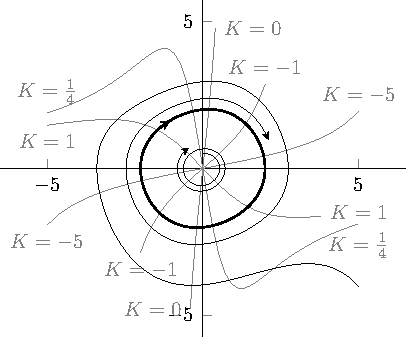
\includegraphics{figSystemVanDerPolEquationA}
\caption{ون ڈر پول مساوات؛ \عددی{\mu=0.1} لیتے ہوئے دو خط حرکت کو تحدیدی دائرہ تک پہنچتے ہوئے دکھایا گیا ہے۔}
\label{شکل_نظام_ون_ڈر_پول_پہلی_شکل}
\end{figure}

شکل \حوالہ{شکل_نظام_ون_ڈر_پول_پہلی_شکل} میں \عددی{\mu} کی کم قیمت \عددی{(\mu=0.1)} کے لئے چند ہم میلان خطوط کو ہلکی سیاہی میں دکھایا گیا ہے۔اس کے علاوہ تحدیدی دائرے کو موٹی لکیر سے ظاہر کیا گیا ہے۔تحدیدی دائرہ تقریباً گول ہے۔ ایک خط حرکت، جو تحدیدی دائرے کے باہر ہے، اور دوسرا خط حرکت، جو تحدیدی دائرے کے اندر  ہے، کو  تحدیدی دائرے تک پہنچتے ہوئے دکھایا گیا ہے۔تحدیدی دائرہ اور نقطہ فاصل کے گرد بند دائرہ (وسط) میں فرق یہ ہے کہ تحدیدی دائرے تک خط حرکت پہنچتی ہے جبکہ وسط کا خط اسی دائرے پر پایا جاتا ہے۔ \عددی{\mu} کی زیادہ قیمت پر تحدیدی دائرہ گول صورت نہیں رکھتا۔ شکل \حوالہ{شکل_نظام_ون_ڈر_پول_دوسری_شکل} میں \عددی{\mu} کی زیادہ قیمت \عددی{(\mu=1)} کے لئے  تمام صورت حال دکھائی گئی ہے جہاں تحدیدی دائرہ گول نہیں ہے۔
\begin{figure}
\centering
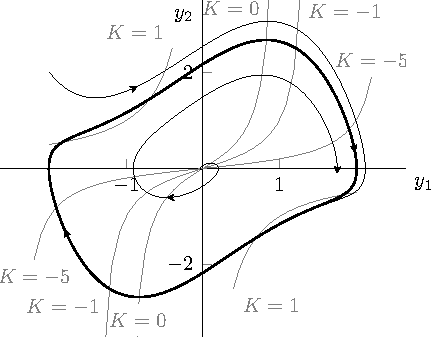
\includegraphics{figSystemVanDerPolEquationB}
\caption{ون ڈر پول مساوات؛ \عددی{\mu=1} لیتے ہوئے دو خط حرکت کو تحدیدی دائرہ تک پہنچتے ہوئے دکھایا گیا ہے۔}
\label{شکل_نظام_ون_ڈر_پول_دوسری_شکل}
\end{figure}
\انتہا{مثال}
%=====================
\ابتدا{مثال}
تفرقی مساوات \عددی{y''+y-y^3=0} سے نظام حاصل کریں۔اس نظام کے تمام نقطہ فاصل دریافت کریں۔نقطہ فاصل کی نوعیت دریافت کریں۔

حل:\عددی{y=y_1} اور \عددی{y'=y_1'=y_2} لیتے ہوئے اور \عددی{y''=y_2'} لکھتے ہوئے دیے گئے دو درجی مساوات سے نظام
\begin{gather}
\begin{aligned}\label{مساوات_مثال_نظام_تفرقی_سے_نظام}
y_1'&=f_1=y_2\\
y_2'&=f_2=-y_1+y_1^3
\end{aligned}
\end{gather}
 حاصل ہوتا ہے۔نقطہ فاصل \عددی{f_1=f_2=0} سے حاصل ہوں گے۔\عددی{f_1=0} سے \عددی{y_2=0} ملتا ہے جبکہ \عددی{f_2=y_1(-1+y_1^2)=0} سے \عددی{y_1=0} اور \عددی{y_1=\mp 1} ملتے ہیں۔یوں نقطہ فاصل \عددی{(0,0)}، \عددی{-1,0} اور \عددی{1,0} ہیں۔نقطہ فاصل \عددی{(0,0)} مرکز پر پایا جاتا ہے لہٰذا اس پر پہلے غور کرتے ہیں۔نقطہ فاصل کی نوعیت جاننے کی خاطر نظام کو خطی بناتے ہیں۔ایسا کوئی بھی جزو جو \عددی{y^m} یا \عددی{y_1^ny_2^q} کی صورت میں لکھا گیا ہو، جہاں \عددی{m \ne 1} جبکہ \عددی{n} اور \عددی{q} کوئی بھی  مستقل ہو سکتے ہیں، غیر خطی ہو گا۔ان غیر خطی اجزاء کو رد کرنے سے خطی نظام حاصل ہوتا ہے۔یوں \عددی{y_2'} کی مساوات میں \عددی{y_1^3} کو رد کرتے ہوئے خطی نظام 
\begin{gather*}
\begin{aligned}
y_1'&=y_2\\
y_2'&=-y_1
\end{aligned}\quad \implies \quad
\begin{aligned}
\bM{y}'=\begin{bmatrix} 0&1\\-1&0 \end{bmatrix}\bM{y}
\end{aligned}
\end{gather*}
حاصل ہو گا جس سے  \عددی{p=a_{11}+a_{22}=0}، \عددی{q=1>0} اور \عددی{\Delta=-4<0} ملتے ہیں لہٰذا نقطہ \عددی{(0,0)} مستحکم وسط ہے۔

آئیں اب نقطہ \عددی{(-1,0)} پر غور کریں۔اس کو مرکز منتقل کرنے کی خاطر نظام \حوالہ{مساوات_مثال_نظام_تفرقی_سے_نظام} میں \عددی{\tilde{y}_1=y_1+1} یعنی \عددی{y_1=\tilde{y}_1-1} اور \عددی{\tilde{y}_2=y_2} پر کرتے ہوئے
\begin{gather*}
\begin{aligned}
\tilde{y}_1'&=\tilde{y}_2\\
\tilde{y}_2'&=-(\tilde{y}_1-1)+(\tilde{y}_1-1)^3
\end{aligned}\implies
\begin{aligned}
\tilde{y}_1'&=\tilde{y}_2\\
\tilde{y}_2'&=2\tilde{y}_1-3\tilde{y}_1^2+\tilde{y}_1^3
\end{aligned}
\end{gather*}
ملتا ہے۔ غیر خطی اجزاء \عددی{\tilde{y}_1^2} اور \عددی{\tilde{y}_1^3} کو رد کرتے ہوئے خطی نظام
\begin{gather*}
\begin{aligned}
\tilde{y}_1'&=\tilde{y}_2\\
\tilde{y}_2'&=2\tilde{y}_1
\end{aligned}\implies 
\begin{aligned}
\tilde{\bM{y}}'=\begin{bmatrix}0&1\\2&0  \end{bmatrix}\tilde{\bM{y}}
\end{aligned}
\end{gather*}
ملتا ہے۔اس سے \عددی{p=0}، \عددی{q=-2<0} اور \عددی{\Delta=8>0} حاصل ہوتے ہیں لہٰذا نقطہ \عددی{(-1,0)} غیر مستحکم نقطہ زین ہے۔

نقطہ \عددی{(1,0)} پر غور کرنے کی  خاطر اس کو مرکز منتقل کرتے ہیں۔ایسا کرنے کی خاطر \عددی{\tilde{y}_1=y_1-1} اور \عددی{\tilde{y}_2=y_2} چنتے ہیں۔یوں نظام
\begin{align*}
\tilde{y}_1'&=\tilde{y}_2\\
\tilde{y}_2'&=2\tilde{y}_1+3\tilde{y}_1^2+\tilde{y}_1^3
\end{align*}
ملتا ہے جس میں غیر خطی اجزاء  \عددی{\tilde{y}_1^2} اور \عددی{\tilde{y}_1^3} رد کرتے ہوئے  خطی نظام
\begin{gather*}
\begin{aligned}
\tilde{y}_1'&=\tilde{y}_2\\
\tilde{y}_2'&=2\tilde{y}_1
\end{aligned}\implies 
\begin{aligned}
\tilde{\bM{y}}'=\begin{bmatrix}0&1\\2&0  \end{bmatrix}\tilde{\bM{y}}
\end{aligned}
\end{gather*}

ملتا ہے۔اس سے \عددی{p=0}، \عددی{q=-2<0} اور \عددی{\Delta=8>0} حاصل ہوتے ہیں لہٰذا نقطہ \عددی{(1,0)} غیر مستحکم نقطہ زین ہے۔
\انتہا{مثال}
%======================

\حصہء{سوالات}
سوال \حوالہ{سوال_نظام_خطی_بنانا_الف} تا سوال \حوالہ{سوال_نظام_خطی_بنانا_ب} کو \موٹا{خطی بناتے} ہوئے تمام نقطہ فاصل دریافت کریں۔ نقطہ فاصل کی نوعیت جدول \حوالہ{جدول_نظام_نقطہ_فاصل_اصول_جانچ} اور جدول \حوالہ{جدول_نظام_نقطہ_فاصل_بالمقابل_استحکام} کی مدد سے دریافت کریں۔

%===============
\ابتدا{سوال}\شناخت{سوال_نظام_خطی_بنانا_الف}\quad 
$y_1'=4y_1-y_1^2,\quad y_2'=y_2$

جوابات:نقطہ فاصل \عددی{f_1=f_2=0} سے \عددی{(0,0)} اور \عددی{(4,0)} حاصل ہوتے ہیں۔مسئلے کو \عددی{(0,0)} پر خطی بناتے ہوئے \عددی{\bM{A}=\begin{bmatrix} 4&0\\0&1  \end{bmatrix}} لکھا جاتا ہے جس سے \عددی{p>0}، \عددی{q>0} اور \عددی{\Delta>0} ملتا ہے لہٰذا نقطہ \عددی{(0,0)} غیر مستحکم جوڑ ہے۔ نقطہ \عددی{(4,0)} کو مرکز پر منتقل کرنے کی خاطر \عددی{\tilde{y}_1=y_1-4} اور \عددی{\tilde{y}_2=y_2} پر کرتے ہیں اور مسئلے کو (\عددی{-\tilde{y}_1^2} رد کرتے ہوئے) خطی بناتے ہوئے \عددی{\bM{A}=\begin{bmatrix} -4&0\\0&1  \end{bmatrix}} حاصل ہوتا ہے جو \عددی{p<0}، \عددی{q<0} اور \عددی{\Delta>0} دیتا ہے  جو غیر مستحکم نقطہ زین کو ظاہر کرتی ہے۔
\انتہا{سوال}
%======================
\ابتدا{سوال}\quad 
$y_1'=y_2,\quad y_2'=-y_1+\frac{2}{3}y_1^2$\\
جوابات:نقطہ فاصل \عددی{f_1=f_2=0} سے \عددی{(0,0)} اور \عددی{(\tfrac{3}{2},0)} حاصل ہوتے ہیں۔نقطہ \عددی{(0,0)} پر مسئلہ خطی بناتے ہوئے \عددی{\bM{A}=\begin{bmatrix} 0&1\\-1&0  \end{bmatrix}} حاصل ہوتا ہے جس سے \عددی{p=0}، \عددی{q>0} اور \عددی{\Delta<0} ملتے ہیں لہٰذا نقطہ \عددی{(0,0)} مستحکم وسط ہے۔ نقطہ \عددی{(\tfrac{3}{2},0)} کو مرکز پر منتقل کرنے کی خاطر \عددی{\tilde{y}_1=y_1-\tfrac{3}{2}} اور \عددی{\tilde{y}_2=y_2} پر کرتے ہیں اور  مسئلے کو (\عددی{\tfrac{2}{3}\tilde{y}_1^2} رد کرتے ہوئے) خطی بنانے سے  \عددی{\bM{A}=\begin{bmatrix} 0&1\\1&0  \end{bmatrix}} حاصل ہوتا ہے لہٰذا \عددی{(\tfrac{2}{3},0)} غیر مستحکم نقطہ زین ہے۔
\انتہا{سوال}
%======================
\ابتدا{سوال}\quad 
$y_1'=y_2,\quad y_2'=-2y_1-y_1^2$\\
جوابات:مستحکم وسط \عددی{(0,0)} پر پایا جاتا ہے جبکہ \عددی{(-2,0)} غیر مستحکم نقطہ زین  ہے۔
\انتہا{سوال}
%======================
\ابتدا{سوال}\quad 
$y_1'=-y_1+y_2+y_1^2,\quad y_2'=-y_1-y_2$\\
جوابات:\عددی{(0,0)} پر مستحکم اور جاذب نقطہ مرغولہ پایا جاتا ہے جبکہ \عددی{(-2,2)} پر غیر مستحکم نقطہ زین پایا جاتا ہے۔
\انتہا{سوال}
%======================
\ابتدا{سوال}\شناخت{سوال_نظام_خطی_بنانا_ب}\quad 
$y_1'=-y_1+y_2-y_2^2,\quad y_2'=-y_1-y_2$\\
جوابات:\عددی{(0,0)} پر جاذب  نقطہ مرغولہ  پایا جاتا ہے جبکہ \عددی{(-2,2)} پر غیر مستحکم نقطہ زین پایا جاتا ہے۔
\انتہا{سوال}
%======================

سوال \حوالہ{سوال_نظام_تفرقی_سے_نظام_الف} تا سوال \حوالہ{سوال_نظام_تفرقی_سے_نظام_ب} میں تفرقی مساوات سے نظام حاصل کریں۔اس نظام کے تمام نقطہ فاصل دریافت کریں۔نظام کو خطی بناتے ہوئے نقطہ فاصل کی نوعیت دریافت کریں۔

%==================
\ابتدا{سوال}\شناخت{سوال_نظام_تفرقی_سے_نظام_الف}\quad 
$y''-4y+y^3=0$\\
جوابات: نظام \عددی{y_1'=y_2} اور \عددی{y_2'=4y_1-y_1^3} حاصل ہوتا ہے۔\عددی{(0,0)} غیر مستحکم نقطہ زین، \عددی{(-2,0)} مستحکم وسط اور \عددی{(2,0)} مستحکم وسط ہیں۔
\انتہا{سوال}
%========================
\ابتدا{سوال}\quad 
$y''+4y-y^3=0$\\
جوابات: نظام \عددی{y_1'=y_2} اور \عددی{y_2'=4y_1-y_1^3} حاصل ہوتا ہے۔\عددی{(0,0)} مستحکم وسط، \عددی{(-2,0)} غیر مستحکم نقطہ زین اور \عددی{(2,0)} غیر مستحکم نقطہ زین ہیں۔
\انتہا{سوال}
%========================
\ابتدا{سوال}\quad 
$y''+4y+y^2=0$\\
جوابات:\عددی{(0,0)} مستحکم وسط اور \عددی{(-4,0)} غیر مستحکم نقطہ زین ہے۔
\انتہا{سوال}
%========================
\ابتدا{سوال}\quad 
$y''+\sin y=0$\\
جوابات: \عددی{(0,0)} اور \عددی{(\mp n2\pi,0)} مستحکم وسط ہیں جہاں \عددی{n=1,2,3,\cdots} ہو سکتا ہے۔نقطہ \عددی{(\mp m\pi,0)} غیر مستحکم نقطہ زین ہے جہاں \عددی{m=1,3,5,\cdots} ہو سکتا ہے۔
\انتہا{سوال}
%========================
\ابتدا{سوال}\شناخت{سوال_نظام_تفرقی_سے_نظام_ب}\quad 
$y''+\cos y=0$\\
جوابات: نقطہ \عددی{(\tfrac{\pi}{2}\mp n2\pi,0)} غیر مستحکم نقطہ نیز  جبکہ \عددی{(-\tfrac{\pi}{2}\mp n2\pi,0)} وسط ہیں جہاں \عددی{n=1,2,3,\cdots} ہو سکتا ہے۔آپ کو \عددی{-\cos(\mp\tfrac{\pi}{2}+\tilde{y}_1)=\sin(\mp \tilde{y}_1)\approx \mp \tilde{y}_1} کی مدد لے سکتے ہیں۔
\انتہا{سوال}
%========================
\ابتدا{سوال}\quad ریلے مساوات\\
\عددی{Y''-\mu(1-\tfrac{1}{3}Y'^2)Y'+Y=0} جہاں \عددی{\mu >0} ہے، \اصطلاح{ریلے مساوات}\فرہنگ{ریلے مساوات}\فرہنگ{مساوات!ریلے}\حاشیہب{Rayleigh equation}\فرہنگ{Rayleigh equation}\فرہنگ{equation!Rayleigh}  کہلاتی\حاشیہد{لارڈ ریلے، جن کا اصل نام جان ولیم سٹرٹ ہے  انگلستان کے ماہر طبیعیات اور ریاضی دان تھے۔} ہے۔اس میں \عددی{y=Y'} پر کرتے ہوئے تفرق لے کر \موٹا{ون در پول مساوات} حاصل کریں۔
\انتہا{سوال}
%====================
\ابتدا{سوال}\quad ڈفنگ مساوات\\
اسپرنگ اور کمیت کی مساوات \عددی{y''+\omega_0^2=0} میں غیر خطی قوت بحالی کی صورت میں \اصطلاح{ڈفنگ مساوات}\فرہنگ{ڈفنگ مساوات}\فرہنگ{مساوات!ڈفنگ}\حاشیہب{Duffing equation}\فرہنگ{equation!Duffing}\فرہنگ{Duffing equation} \عددی{y''+\omega_0^2y+\beta y^3=0} حاصل ہوتی ہے جہاں \عددی{\abs{\beta}} عموماً چھوٹی مقدار ہوتی ہے۔\عددی{\beta>0} کو \ترچھا{سخت اسپرنگ} اور \عددی{\beta<0} کو \ترچھا{نرم اسپرنگ} کی صورت پکارا جاتا ہے۔سطح حرکت پر خط حرکت کی مساوات دریافت کریں۔

جواب:\عددی{2y_2^2+2\omega_0^2y_1^2+\beta y_1^4=K} جہاں \عددی{K} مستقل مقدار ہے۔
\انتہا{سوال}
%====================
\ابتدا{سوال}\quad خط حرکت\\
سادہ تفرقی مساوات \عددی{y''-9y+y^3=0} کو نظام کی صورت میں لکھیں جس کو حل کرتے ہوئے \عددی{y_2} بالمقابل \عددی{y_1} کی مساوات حاصل کریں۔حاصل مساوات سے سطح حرکت پر چند خط حرکت کھینچیں۔

جواب:\عددی{2y_2^2=18y_1^2-y_1^4+K} جہاں \عددی{K} مستقل مقدار ہے۔
\انتہا{سوال}
%=====================

\حصہ{سادہ تفرقی مساوات کے غیر متجانس خطی نظام}
اس حصے میں غیر متجانس نظام
\begin{align}\label{مساوات_نظام_غیر_متجانس_مساوات_الف}
\bM{y}'=\bM{A}\bM{y}+\bM{g}\quad \quad \text{\RL{(حصہ \حوالہ{حصہ_نظام_نظریہ_نظام} دیکھیں)}}
\end{align}
جہاں \عددی{\bM{g}} غیر صفر سمتیہ  ہے، کو حل کرنا سیکھتے ہیں۔ہم فرض کرتے ہیں کہ \عددی{\bM{g}(t)} اور \عددی{n \times n} قالب \عددی{\bM{A}(t)} کے ارکان،  محور \عددی{t} کے کھلے وقفہ \عددی{J} پر استمراری ہیں۔وقفہ \عددی{J} پر متجانس مساوات \عددی{\bM{y}'=\bM{A}\bM{y}} کے عمومی حل \عددی{\bM{y}^{(h)}(t)} اور \عددی{J} پر مساوات \حوالہ{مساوات_نظام_غیر_متجانس_مساوات_الف} کے کسی بھی \اصطلاح{مخصوص حل}\فرہنگ{مخصوص حل}\فرہنگ{particular solution} \عددی{\bM{y}^{(p)}(t)} [جس میں کوئی مستقل نہیں پایا جاتا] سے مساوات \حوالہ{مساوات_نظام_غیر_متجانس_مساوات_الف} کا \عددی{J} پر \اصطلاح{عمومی حل}\فرہنگ{عمومی حل}\فرہنگ{حل!عمومی}\فرہنگ{general!solution}
\begin{align}
\bM{y}=\bM{y}^{(h)}+\bM{y}^{(p)}
\end{align}
حاصل ہوتا ہے۔مسئلہ \حوالہ{مسئلہ_نظام_خطی_نظام_وجودیت_یکتائی} کے تحت عمومی حل \عددی{\bM{y}} میں \عددی{J} پر مساوات \حوالہ{مساوات_نظام_غیر_متجانس_مساوات_الف} کے تمام ممکنہ حل شامل ہیں۔

متجانس مساوات کے حل پر ہم گزشتہ حصوں میں غور کر چکے ہیں۔اس حصے میں غیر متجانس مساوات کے مخصوص حل کے حصول پر غور کرتے ہیں۔نا معلوم عددی سر کی ترکیب اور مقدار معلوم بدلنے کے طریقوں پر غور کرتے ہیں جنہیں ہم حصہ \حوالہ{حصہ_سادہ_دو_غیر_متجانس} اور حصہ \حوالہ{سادہ_دو_متغیرات_بدلنے_کا_طریقہ} سے جانتے ہیں۔ 
%=============

\جزوحصہ{نا معلوم عددی سر کی ترکیب}
 ایک عدد سادہ تفرقی مساوات کے حل میں استعمال ہونے کی طرح اب بھی یہ ترکیب اس صورت  قابل استعمال ہو گی جب  \عددی{\bM{A}} کے ارکان مستقل مقدار ہوں  اور \عددی{\bM{g}} کی قیمت مستقل مقدار ہو، \عددی{t^m} تفاعل ہوں جہاں \عددی{m} مثبت اعداد ہیں، قوت نمائی تفاعل ہوں، سائن  اور کوسائن تفاعل ہوں۔ایسی صورت میں مخصوص حل کو \عددی{\bM{g}} کی طرح تصور کیا جاتا ہے لہٰذا \عددی{\bM{g}=t^2} ہونے کی صورت میں \عددی{\bM{y}^{(p)}=\bM{u}+\bM{v}t+\bM{w}t^2} فرض کیا جائے گا۔ مساوات \حوالہ{مساوات_نظام_غیر_متجانس_مساوات_الف} میں \عددی{\bM{y}^{(p)}} پر کرتے ہوئے \عددی{\bM{u}}،  \عددی{\bM{v}} اور \عددی{\bM{w}} حاصل کیے جاتے ہیں۔یہ حصہ \حوالہ{حصہ_سادہ_دو_غیر_متجانس} کی طرح ہے البتہ یہاں ترمیمی قاعدہ قدر مختلف ہے۔ آئیں ایک مثال کی مدد سے اس ترکیب کا استعمال دیکھیں۔
%================

\ابتدا{مثال}\شناخت{مثال_نظام_غیر_متجانس_نا_معلوم_سر}\quad نا معلوم عددی سر کی ترکیب۔ترمیمی قاعدہ\\
درج ذیل مساوات کی عمومی حل حاصل کریں۔
\begin{align}\label{مساوات_مثال_غیر_متجانس_نا_معلوم_سر_الف}
\bM{y}'=\bM{A}\bM{y}+\bM{g}=\begin{bmatrix*}[r] -2&1\\1&-2 \end{bmatrix*} \bM{y}+\begin{bmatrix*}[r] -4\\3 \end{bmatrix*} e^{-3t}
\end{align}

حل:ہم صفحہ \حوالہصفحہ{مثال_نظام_خط_حرکت_غیر_مناسب} پر مثال \حوالہ{مثال_نظام_خط_حرکت_غیر_مناسب} میں نظیری متجانس مساوات کا حل 
\begin{align}\label{مساوات_مثال_غیر_متجانس_نا_معلوم_سر_ب}
\bM{y}=c_1\begin{bmatrix} 1 \\ 1 \end{bmatrix}e^{-t}+c_2\begin{bmatrix*}[r] 1\\ -1 \end{bmatrix*}e^{-3t}
\end{align}
حاصل کر چکے ہیں۔چونکہ \عددی{\bM{A}} کا  \عددی{\lambda=-3} آئگنی قدر ہے اور مساوات \حوالہ{مساوات_مثال_غیر_متجانس_نا_معلوم_سر_الف} میں دائیں جانب \عددی{e^{-3t}} پایا جاتا ہے لہٰذا  اس جزو کو \عددی{t} سے ضرب دیتے ہوئے \عددی{\bM{y}^{(h)}} میں شامل کرتے ہیں۔
\begin{align}\label{مساوات_مثال_غیر_متجانس_نا_معلوم_سر_پ}
\bM{y}^{(h)}=\bM{u}te^{-3t}+\bM{v}e^{-3t} \quad \quad 
\end{align} 
\عددی{\bM{y}^{(h)}} میں بائیں ہاتھ کا پہلا جزو حصہ \حوالہ{حصہ_سادہ_دو_غیر_متجانس} میں دیے گئے  ترمیمی قاعدے کا مماسی قاعدہ ہے، جو یہاں نا کافی ہے۔[آپ کوشش کر کے دیکھ سکتے ہیں]۔ مساوات \حوالہ{مساوات_مثال_غیر_متجانس_نا_معلوم_سر_پ} کو مساوات \حوالہ{مساوات_مثال_غیر_متجانس_نا_معلوم_سر_الف} میں پر کرتے ہیں۔
\begin{align*}
\bM{y}^{(p)'}=\bM{u}e^{-3t}-3\bM{u}te^{-3t}-3\bM{v}e^{-3t}=\bM{A}\bM{u}te^{-3t}+\bM{A}\bM{v}e^{-3t}+\bM{g}
\end{align*}
دونوں جانب \عددی{te^{-3t}} والے اجزاء کے عددی سر برابر ہوں گے لہٰذا \عددی{-3\bM{u}=\bM{A}\bM{u}} ہو گا۔یوں \عددی{\bM{A}} قالب کے آئگنی قدر \عددی{\lambda=-3} کا نظیری آئگنی سمتیہ \عددی{\bM{u}} ہو گا۔اس طرح \عددی{\bM{u}=a[1\quad -1]^T} لکھا جا سکتا ہے جہاں \عددی{a} کوئی بھی غیر صفر مستقل ہو سکتا ہے۔بقایا اجزاء کے عددی سر برابر لکھ کر
\begin{gather*}
\begin{aligned}
\bM{u}-3\bM{v}=\bM{A}\bM{v}+\bM{g}
\end{aligned}\implies
\begin{aligned}
\begin{bmatrix*}[r] a\\-a  \end{bmatrix*}-\begin{bmatrix} 3v_1\\3v_2 \end{bmatrix}=\begin{bmatrix*}[r] -2v_1+v_2\\v_1-2v_2 \end{bmatrix*}+\begin{bmatrix*}[r] -4\\3 \end{bmatrix*}
\end{aligned} 
\end{gather*}
ترتیب دیتے ہیں۔
\begin{align*}
v_1+v_2&=a+4\\
v_1+v_2&=-a-3
\end{align*}
دوسری مساوات کو پہلی سے منفی کرتے ہوئے \عددی{2a+7=0} یعنی \عددی{a=-\tfrac{7}{2}} ملتا ہے۔یوں درج بالا میں پہلی مساوات \عددی{v_1+v_2=-\tfrac{7}{2}+4=\tfrac{1}{2}} ہو گی جس  میں  \عددی{v_1=k} لیتے ہوئے  \عددی{v_2=\tfrac{1}{2}-k} حاصل ہوتا ہے۔اس طرح \عددی{\bM{v}=[k\quad \tfrac{1}{2}-k]^T} ہو گا۔ہم \عددی{k=0} چن سکتے ہیں۔ایسا ہی کرتے ہوئے عمومی حل لکھتے ہیں۔
\begin{align}
\bM{y}=\bM{y}^{(h)}+\bM{y}^{(p)}=\bM{y}=c_1\begin{bmatrix} 1 \\[1em] 1 \end{bmatrix}e^{-t}+c_2\begin{bmatrix*}[r] 1\\[1em] -1 \end{bmatrix*}e^{-3t}-\frac{7}{2}\begin{bmatrix*}[r] 1\\[1em] -1 \end{bmatrix*}te^{-3t}+\begin{bmatrix} 0\\[1em]\frac{1}{2} \end{bmatrix}e^{-3t}
\end{align}
\انتہا{مثال}
%====================
\جزوحصہء\quad مقدار معلوم بدلنے کی ترکیب\\
اس ترکیب سے غیر متجانس نظام
\begin{align}\label{مساوات_نظام_غیر_متجانس_مقدار_معلوم_الف}
\bM{y}'=\bM{A}(t)+\bM{g}(t)
\end{align}
کو حل کیا جا سکتا ہے جہاں \عددی{\bM{A}(t)} متغیر مقدار ہیں اور \عددی{\bM{g}(t)} کوئی بھی تفاعل ہو سکتا ہے۔اگر \عددی{t} محور کے کسی کھلے وقفے \عددی{J} پر  نظیری متجانس نظام کا عمومی حل \عددی{\bM{y}^{(h)}} معلوم ہو تب اس ترکیب کی مدد سے اس وقفے پر نظام \حوالہ{مساوات_نظام_غیر_متجانس_مقدار_معلوم_الف} کا مخصوص حل \عددی{\bM{y}^{(p)}} حاصل کیا جاتا ہے۔آئیں مثال \حوالہ{مثال_نظام_غیر_متجانس_نا_معلوم_سر} کو اس ترکیب سے حل کریں۔
%=================
\ابتدا{مثال}\quad مقدار معلوم بدلنے کے طریقے سے حل\\
گزشتہ مثال کے نظام \حوالہ{مساوات_مثال_غیر_متجانس_نا_معلوم_سر_الف} کو مقدار معلوم بدلنے کی ترکیب سے حل کریں۔
\begin{align}
\bM{y}'=\bM{A}\bM{y}+\bM{g}=\begin{bmatrix*}[r] -2&1\\1&-2 \end{bmatrix*} \bM{y}+\begin{bmatrix*}[r] -4\\3 \end{bmatrix*} e^{-3t}
\end{align}

حل:متجانس مساوات کے حل کی اساس \عددی{[e^{-t}\quad e^{-t}]^T}، \عددی{[e^{-3t}\quad -e^{-3t}]^T} ہے جس سے درج ذیل عمومی حل لکھا جاتا ہے۔
\begin{align}\label{مساوات_نظام_مقدار_معلوم_وائے}
\bM{y}=\begin{bmatrix*}[r] e^{-t}&e^{-3t} \\ e^{-t} &-e^{-3t} \end{bmatrix*} \begin{bmatrix} c_1\\c_2 \end{bmatrix}=\bM{Y}(t)\bM{c}
\end{align}
یہاں \عددی{\bM{Y}(t)=[\bM{y}^{(1)} \quad \bM{y}^{(2)}]^T} بنیادی قالب [حصہ \حوالہ{حصہ_نظام_نظریہ_نظام} دیکھیں] ہے ۔ حصہ \حوالہ{سادہ_دو_متغیرات_بدلنے_کا_طریقہ} کی طرح ہم مستقل سمتیہ \عددی{\bM{c}} کی جگہ متغیر سمتیہ \عددی{\bM{u}} پر کرتے ہوئے مخصوص حل \عددی{\bM{y}^{(p)}} لکھتے ہیں۔
\begin{align}
\bM{y}^{(p)}=\bM{Y}(t)\bM{u}(t)
\end{align}
نظام \حوالہ{مساوات_مثال_غیر_متجانس_نا_معلوم_سر_الف} میں \عددی{\bM{y}^{(p)}} پر کرتے ہیں۔
\begin{align}\label{مساوات_نظام_بنیادی_نظام_الف}
\bM{Y}'\bM{u}+\bM{Y}\bM{u}'=\bM{A}\bM{Y}\bM{u}+\bM{g}
\end{align}
اب چونکہ \عددی{\bM{y}^{(1)}} اور \عددی{\bM{y}^{(2)}} متجانس نظام کا حل ہے لہٰذا \عددی{\bM{y}^{(1)'}=\bM{A}\bM{y}^{(1)}} اور
 \عددی{\bM{y}^{(2)'}=\bM{A}\bM{y}^{(2)}} یعنی \عددی{\bM{Y}'=\bM{A}\bM{Y}}ہو گا۔یوں \عددی{\bM{Y}'\bM{u}=\bM{A}\bM{Y}\bM{u}} لکھ کر مساوات \حوالہ{مساوات_نظام_بنیادی_نظام_الف} سے  \عددی{\bM{Y}\bM{u}'=\bM{g}} حاصل ہوتا ہے جس کا حل درج ذیل ہے۔
\begin{align}
\bM{u}'=\bM{Y}^{-1}\bM{g}
\end{align}
درج بالا اس حقیقت کی بنیاد پر لکھا گیا ہے کہ چونکہ \عددی{\bM{Y}} کا امتیازی مقطع دراصل ورونسکی [حصہ \حوالہ{حصہ_نظام_قالب} دیکھیں] \عددی{W} ہے جو اساس کی صورت میں غیر صفر ہوتا ہے لہٰذا \عددی{\bM{Y}^{-1}} حاصل کیا جا سکتا ہے۔ معکوس قالب کو مساوات \حوالہ{مساوات_نظام_معکوس_قالب} کی مدد سے حاصل کرتے ہوئے
\begin{align*}
\bM{Y}^{-1}=\frac{1}{-2e^{-4t}}\begin{bmatrix} -e^{-3t} & -e^{-3t}\\[1em] -e^{-t}& e^{-t} \end{bmatrix}=
\frac{1}{2}\begin{bmatrix} e^{t} & e^{t}\\[1em] e^{3t}& -e^{3t}   \end{bmatrix}
\end{align*}
\عددی{\bM{g}} سے ضرب دیتے ہوئے \عددی{\bM{u}'} لکھتے ہیں۔
\begin{align*}
\bM{u}'=\bM{Y}^{-1}\bM{g}=\frac{1}{2}\begin{bmatrix} e^{t} & e^{t}\\[1em] e^{3t}& -e^{3t}   \end{bmatrix}\begin{bmatrix} -4e^{-3t} \\[1em] 3e^{-3t} \end{bmatrix} =\begin{bmatrix}-\frac{1}{2}e^{-2t}\\[1em] -\frac{7}{2}\end{bmatrix}
\end{align*}
\عددی{\bM{u}} حاصل کرنے کی خاطر تکمل لیتے ہیں۔تفرق کی طرح ہر جو کا علیحدہ تکمل لیا جاتا ہے۔
\begin{align*}
\bM{u}(t)=\int_{0}^{t}\begin{bmatrix}-\frac{1}{2}e^{-2t}\\[1em] -\frac{7}{2}\end{bmatrix}=\begin{bmatrix} \frac{1}{4}(e^{-2t}-1) \\[1em] -\frac{7}{2}t \end{bmatrix}
\end{align*}
یوں مساوات \حوالہ{مساوات_نظام_مقدار_معلوم_وائے} کی مدد سے درج ذیل لکھا جا سکتا ہے۔
\begin{align*}
\bM{Y}\bM{u}=\begin{bmatrix*}[r] e^{-t}&e^{-3t} \\ e^{-t} &-e^{-3t} \end{bmatrix*}\begin{bmatrix} \frac{1}{4}(e^{-2t}-1) \\[1em] -\frac{7}{2}t \end{bmatrix}=\begin{bmatrix}\frac{1}{4}e^{-3t}-\frac{1}{4}e^{-t}-\frac{7}{2}te^{-3t}\\[1em] \frac{1}{4}e^{-3t}-\frac{1}{4}e^{-t}+\frac{7}{2}te^{-3t}  \end{bmatrix}=\begin{bmatrix} \frac{1}{4}-\frac{7}{2}t \\[1em] \frac{1}{4}+\frac{7}{2}t \end{bmatrix}e^{-3t}-\begin{bmatrix}\frac{1}{4}\\[1em] \frac{1}{4}  \end{bmatrix}e^{-t}
\end{align*}
اس مساوات کے بائیں ہاتھ آخری جزو متجانس مساوات کا حل ہے لہٰذا اس جزو کو متجانس مساوات کے حل \عددی{\bM{y}^{(h)}} میں ضم کیا جا سکتا ہے۔یوں بقایا حصے کو \عددی{\bM{y}^{(p)}} لیتے ہوئے عمومی حل لکھتے ہیں۔
\begin{align}
\bM{y}=\bM{y}^{(h)}+\bM{y}^{(p)}=c_1\begin{bmatrix}1\\1  \end{bmatrix}e^{-t}+c_2\begin{bmatrix*}[r]1\\-1  \end{bmatrix*}e^{-3t}+\frac{1}{4} \begin{bmatrix}1\\1  \end{bmatrix}e^{-3t}-\frac{7}{2}\begin{bmatrix*}[r]1\\ -1  \end{bmatrix*}te^{-3t}
\end{align}
\انتہا{مثال}
